\documentclass[a4paper,11pt]{report}

\usepackage{caption}
\usepackage{courier}
\usepackage{url}
\usepackage{graphicx}
\usepackage{amssymb,amstext,amsmath}
\usepackage{pstricks}
\usepackage{lscape}
\usepackage{rotating}
\usepackage{pst-node}
\usepackage{listings}
\usepackage{makeidx}
\usepackage{pst-blur}
\usepackage{geometry}
\usepackage{times} 
\usepackage{setspace}
\usepackage{algorithmic}
\usepackage{algorithm}
\DeclareCaptionFont{white}{\color{white}}
\DeclareCaptionFormat{listing}{\colorbox[cmyk]{0.43, 0.35, 0.35,0.01}{\parbox{\textwidth}{\hspace{15pt}#1#2#3}}}
\captionsetup[lstlisting]{format=listing,labelfont=white,textfont=white, singlelinecheck=false, margin=0pt, font={bf,footnotesize}}
\setlength{\parindent}{-3pt}
%
\begin{document}
%----------------------------------------------------------
%\renewcommand{\chaptermark}[1]{\markboth{\MakeUppercase{#1}}{}}
%\renewcommand\chaptername{Test}
%----------------------------------------------------------
\lstset{
         basicstyle=\footnotesize\ttfamily, % Standardschrift
         %numbers=left,               % Ort der Zeilennummern
         numberstyle=\tiny,          % Stil der Zeilennummern
         %stepnumber=2,               % Abstand zwischen den Zeilennummern
         numbersep=5pt,              % Abstand der Nummern zum Text
         tabsize=2,                  % Groesse von Tabs
         extendedchars=true,         %
         breaklines=true,            % Zeilen werden Umgebrochen
         keywordstyle=\color{red},
            frame=b,         
 %        keywordstyle=[1]\textbf,    % Stil der Keywords
 %        keywordstyle=[2]\textbf,    %
 %        keywordstyle=[3]\textbf,    %
 %        keywordstyle=[4]\textbf,   \sqrt{\sqrt{}} %
         stringstyle=\color{white}\ttfamily, % Farbe der String
         showspaces=false,           % Leerzeichen anzeigen ?
         showtabs=false,             % Tabs anzeigen ?
         xleftmargin=17pt,
         framexleftmargin=17pt,
         framexrightmargin=5pt,
         framexbottommargin=4pt,
         %backgroundcolor=\color{lightgray},
         showstringspaces=false      % Leerzeichen in Strings anzeigen ?        
 }
 \lstloadlanguages{% Check Dokumentation for further languages ...
         %[Visual]Basic
         %Pascal
         C
         %C++
         %XML
         %HTML
         %Java
 }
    %\DeclareCaptionFont{blue}{\color{blue}} 


%\lstset{ %
%language=C++,                % choose the language of the code
%basicstyle=\footnotesize,       % the size of the fonts that are used for the code
%numbers=left,                   % where to put the line-numbers
%numberstyle=\footnotesize,      % the size of the fonts that are used for the line-numbers
%stepnumber=5,                   % the step between two line-numbers. If it's 1 each line will be numbered
%numbersep=5pt,                  % how far the line-numbers are from the code
%%backgroundcolor=\color{},  % choose the background color. You must add \usepackage{color}
%showspaces=false,               % show spaces adding particular underscores
%showstringspaces=false,         % underline spaces within strings
%keywordstyle=\color{green},
%showtabs=false,                 % show tabs within strings adding particular underscores
%frame=single,           % adds a frame around the code
%tabsize=2,          % sets default tabsize to 2 spaces
%captionpos=b,           % sets the caption-position to bottom
%breaklines=true,        % sets automatic line breaking
%breakatwhitespace=false,    % sets if automatic breaks should only happen at whitespace
%escapeinside={\%*}{*)}          % if you want to add a comment within your code
%}
%-----------------------------------------------------------
\begin{titlepage}
 
\begin{center}

\ \\[1.5cm] 
\textbf{\Large DEDUPLICATION AND COMPRESSION BENCHMARKING SUPPORT IN FILEBENCH}\\[1.5cm]
 
 \textbf{ \small CSE506 Project Report}\\[1.5cm]

\textbf{By\\Rami Al-Rfou'\\ Nikhil Patwardhan \\ Phanindra Bhagavatula}\\[1.5cm]
{\textit{ \today}} 


\end{center}
\vfill
\end{titlepage}

%-----------------------------------------------------------
\tableofcontents
%-----------------------------------------------------------
Deduplication systems look for repeating patterns of data at the block and bit levels. When multiple instances of the same pattern are discovered, the system stores a single copy of the pattern. However, most of the popular file-system benchmarks generate data in a manner that does not enable realistic benchmarking of deduplication systems. Controlling the entropy of the data that is used while benchmarking deduplication systems is one way of overcoming this limitation. In this project, we integrated entropy-based data generation in the Filebench file-system benchmarking suite.

By assuming the emission of a byte in the data stream as an event, we generate data that can take values from 0 to 8 bits/byte. The user is able to control the value of entropy by specifying it in the workload to be run. We show that by varying the amount of entropy of data that is either written to or read from a disk using a deduplicated file-system, the benchmarking results are more pertinent to the actual behavior of such a file-system.

\chapter{Introduction}\label{chap:intro}

\section{Filebench}
\paragraph{}
Filebench is a framework for simulating different file systems workloads. Such simulation is
helpful to identify performance weaknesses and bottlenecks in file systems. 
Filebench interface relies on an interpreter that reads workload Definition language scenarios in \verb+f+ scripts files.
The model language is expressive which allows Filebench to run so complicated
testing workloads. Filebench at the same time hides the complexity of running multi threaded systems and synchronizing them. Moreover, it offers
an integrated system to measure the latency and throughput for each operation\cite{web:fb-main}.

\paragraph{}
Nowadays, complex applications such as relational databases have sophisticated relations in the system. Setting up each 
application in environment that already has other applications can complicate the benchmarking 
and make it hard to evaluate the results. Filebench gives the power to simulate an application from the
perspective of the filesystem isolating any other interactions that the application can have with other
components of the system.


\section{SDFS}

\paragraph{}
Deduplication becomes more important because of the new features 
that nowadays file systems are offerings as backups and snapshots.
Such features keeps a lot of redundant data on the storage medium.
Cloud computing is forcing more challenges on file systems running
on servers in terms of scalability and storage footprint. Many
of the virtualization environments are keeping copies of the operating systems
images running on the system. Most of those images are similar to large extent
that deduplication can be so useful\cite{usenix}.

\paragraph{}
SDFS is a open source project to implement a file system with deduplication support. Deduplication is a technique
used to save disk space by keeping track of redundant data and save only one copy of that data. Deduplication differs
from compression that the scope of redundancy that has to be avoided is across the file system and on file or at
 least chunks of the file basis. On the other hand compression tries to reduce the size of a file by looking at its byte stream.

\paragraph{}
SDFS offers two mechanism to achieve deduplication: inline and batch mechanisms. The inline mechanism stores chunks of the files and
take a finger print of each chunk by calculating the hash function of the data and then write it directly to storage medium. In case
a similar chunk or file has to be written again, SDFS does not write it instead just references to the existing chunk on the disk.
The batch mode applies a post-process deduplication. The data is stored directly to the disk then the file system perdiodically checks 
for any chance of duplicated chunks.



\paragraph{}
SDFS is implemented as a userspace file system and it is written in JAVA. This gives flexibility to use SDFS without updating the system.
Beside that implementing it in JAVA makes it easier to support multiple operating systems.
\begin{figure}
\label{fig:fuse}
\begin{center}
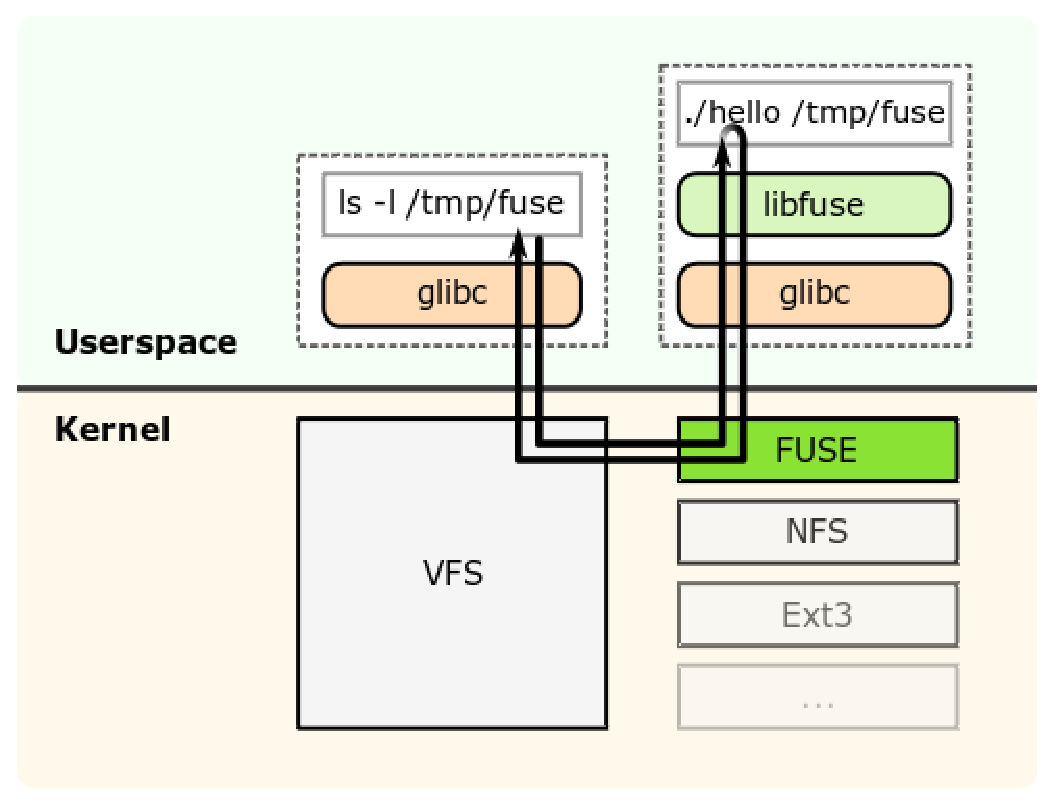
\includegraphics[scale=.55]{FUSE.eps}
\caption{Userspace file system architecture in linux\cite{web:wiki-fuse}}
\end{center}
\end{figure}

\paragraph{}
From figure \ref{fig:fuse}, it is clear the userspace file systems has a lot of similarity of stackable file systems. They allow the developer
to add functionality to an existing file system without changing it. Moreover, they give the flexibility to make such improvements without 
updating the operating system. Userspace performance may suffer due to the extra communication overhead and context switching between kernel and userspace.
However, it has a security advantage by reducing the size of code base runs in the kernel mode.

\begin{figure}[H]
\label{fig:sdfsarch}
\begin{center}
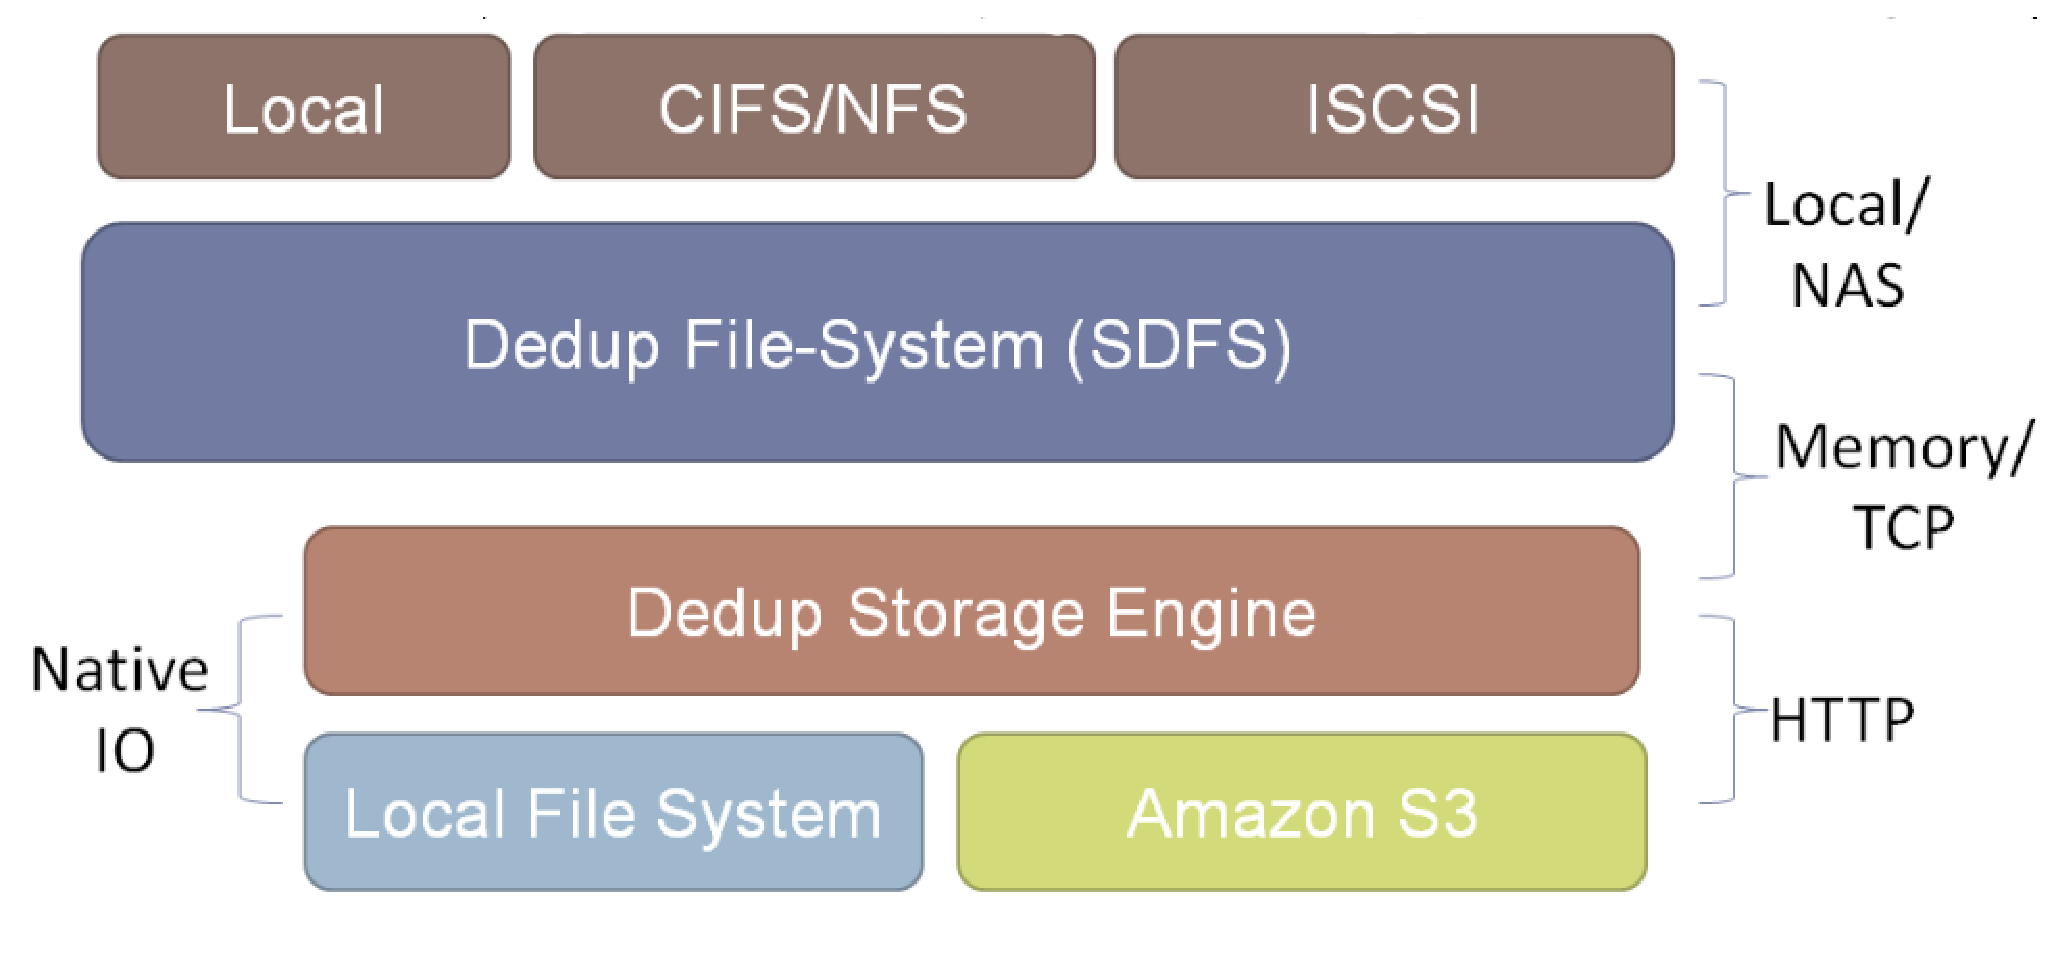
\includegraphics[scale=0.30]{sdfs_arch.eps}
\caption{SDFS Architecture\cite{web:opendedup}}
\end{center}
\end{figure}

\paragraph{}
Figure \ref{fig:sdfsarch} shows that SDFS has a server client design model. The client can be a process on the host machine or a network socket that
writes data to the disk. SDFS integrates with NFS and VFS to support network and local operations. 


\chapter{Design}\label{chap:des}

\paragraph{}
Currently Filebench initialize the files contents by assigning the files uninitialized memory segments.
 To control the entropy of the data written to the disk, we have to communicate more files data specific information to Filebench operations.

\paragraph{}
As the information we want to send to Filebench operations is data specific, it was ituitive to combine as this information as attributes to the structure that already keeps track of the files properities, \verb+fileset+.
Making the entropy as attribute of the filesets and not a global variable in the \verb+f+ scenario script gives us the flexibility to have filesets with different entropies.\\

\section{Filebench Interpreter}
The changes in the Filebench Interpreter have been designed to enable Filebench to optionally accept various datasources. These datasources are meant to be used to populate files created during benchmarking process. The Interpreter has thus been modified to accept new attributes called \verb+datasource+ and \verb+entropy+ as a part of the fileset command. For example a valid fileset command is:\\

\indent \verb+define fileset name=bigfileset,...,datasource=entro,entropy=3.4+
\paragraph{}
The attribute \verb+entropy+ is not directly an attribute of \verb+fileset+ command. It is a subattribute of the datasource type. For example the below is an invalid fileset definition.\\

\verb+define fileset name=bigfileset,path=\$dir,...,entropy=3.4+\\
\paragraph{}
All attributes for command \verb+fileset+ have a place in the \verb+struct fileset+. The \verb+datasouce+ attribute has also been placed in the structure. A new place has been created in this structure for \verb+datasource+ attribute alone and not for \verb+entropy+ attribute. The logic is that, the only attribute that makes sense to be part of \verb+fileset+ is the type of data defined by datasource. The attributes which define the data itself of the \verb+datasource+ are irrelevant to be part of \verb+fileset+ datastructure.
\paragraph{}
Since the a datasource can have various attributes of the data constituting it, \verb+datasource+ object has a pointer to a list of attribute objects relevant to it. This is the reason \verb+datasource+ is of type \verb+attr+ and not \verb+avd_t+. To accommodate  a list of sub-attributes inside an attribute(like the \verb+datasource+), \verb+struct attr+ has been modified.
\documentclass{article}
\begin{document}
\section{Integration of entropy functionality in Filebench}
The design can be logically divided into the following parts:

\subsection{Data Specification}
Data intended to be written to or read from files could be specified in many ways for benchmarking purposes. One approach is by specifying its \textit{entropy}. However, in future, users may have more specific requirements like populating a certain character in the data or a specific distribution for the data. We currently support only entropy based data population, but keeping possible future requirements in mind we chose to create a separate structure which is dedicated to store all the specifications about the data itself. One of its fields is a function pointer that is set \textit{dynamically} depending on the type of data  requested. Since data specification is made per \textit{fileset}, we put this structure as a member of \texttt{struct fileset}.

\subsection{Fileset Initialization}
The \texttt{struct fileset} structure holds information that is relevant to a set of files. Entropy is specified per \textit{fileset} and it is recorded in this structure by the parser, as explained in section \_\_\_HERE\_\_\_. This information is used to appropriately initialize the structure described above. Its function pointer is dynamically pointed to a function that provides data in the desired format. Once initialized, this function pointer can be used by the corresponding \textit{flow operations} to populate their buffers in a generic manner.

\subsection{Flow Operations}
Flow operations represent workload actions and they carry out buffered I/O on the files. Using the dynamically set function pointer, we populate the buffer (in this case with the specified entropy) just before writing it to an open file in the following flow operations:
\begin{enumerate}
\item write
\item writewholefile
\item appendfile
\item appendfilerand
\end{enumerate}
\end{document}
\section{Entropy Generator}\label{sec:ent_des}
\subsection{Entropy function}\label{sub:func}
The entropy is quantity that is defined for a set of data to quantify how much random it is.
For any stream of data that is composed of $n$ symbols, its entropy is given by the following
equation:
\begin{equation}\label{eq:ent}
Entropy = -\sum_{i=1}^n P(s_i)\lg P(s_i)
\end{equation}

$P(s_i)$ is the probability that a symbol $s_i$ is generated by the data generator.
To calculate the probability of a symbol in a generated data, can be done by calculating
the experimental probability according to equation \ref{eq:exp}
\begin{equation}\label{eq:exp}
P(s) = \frac{number\, of\, s\, occurences}{size\, of\, data}
\end{equation}

The maximum entropy that can be obtained from a data generated using $n$ symbols is when the
probability distribution of symbols is uniform. That entropy of a uniform distribution can by calculated as following
\begin{align}
Entropy &= -\sum_{i=1}^n P(s_i)\lg P(s_i) \nonumber \\
        &= -\sum_{i=1}^n \frac{1}{n} \lg \frac{1}{n} \nonumber \\
        &= \frac{-1}{n}\sum_{i=1}^n -\lg n \nonumber \\
        &= \lg n 
\end{align}

To decrease the value of entropy, we can imbalance the uniform distribution. Using this method we can reach zero by increasing the probability of the first symbol to 1 and decreasing the
others to zero. However, calculating the $\epsilon_i$ that should be added to subtracted from every $P(s_i)$
to reach a specific entropy value less than $\lg n$ can be hard. To simplify the situation we 
can focus on changing the probability of two symbols at a time.
Our target to generate all values of $x \ni \lg(n-1)<x<\lg n$ just by changing the probability of two symbols.

\begin{align}
Entropy &= -[(P(s_1)+\epsilon)\lg (P(s_1)+\epsilon) + (P(s_2)-\epsilon)\lg (P(s_2)-\epsilon)\nonumber \\
        &\qquad{} +  \sum_{i=3}^n P(s_i)\lg (P(s_i))]\label{eq:imb_ent}\\
 &= -[(\frac{1}{n}+\epsilon)\lg (\frac{1}{n}+\epsilon) + (\frac{1}{n}-\epsilon)\lg (\frac{1}{n}-\epsilon) \nonumber \\
      &\qquad  +  \frac{n-2}{n}\lg (\frac{1}{n})]\label{eq:imb_ent2}
\end{align}


To prove that the entropy as a function of $\epsilon$ equal to any value between $\lg n, \lg (n-1)$, the maximum entropy using $n$, $n-1$ symbols respectively. We notice the following observations:\\
\begin{itemize}
\item Equation \ref{eq:imb_ent2} shows that entropy is a function in one variable, $\epsilon$.
\item Equation \ref{eq:imb_ent2} also shows that the entropy is a continuous function of $\epsilon$ on the interval $\epsilon \in [0,1/n)$ as it is a result of adding and multiplying continuous functions on the same interval.
\item Entropy is equal $\lg n$ when $\epsilon = 0$.
\item Entropy is equal to $\lg(n) -\frac{2}{n}$  when $\epsilon$ reaches $1/n$
\item $\lg(n) - \frac{2}{n} < \lg(n-1) \,\,\, \forall n > 2$ \footnote{Can be verified by visiting\\ 
\url{http://www.wolframalpha.com/input/?i=lg\%28n-1\%29+-+\%28lg\%28n\%29++-+2\%2Fn\%29&a=*FunClash.lg-_*Log2.Log10-}}.
\end{itemize}
Given the above and using the median value theorem the Entropy function spans over the interval $(\lg (n-1), \lg n)$ using subinterval of $\epsilon$ values.
To get the value of $\epsilon$ we can apply any numerical method to find the roots of the equation.

\subsection{Random generator}\label{sub:gen_des}
In \ref{sub:func} we showed that any entropy value can be obtained using a slightly modified uniform distribution.
Now, given that the probability distribution function (PDF) of our symbols is already calculated.
How can we build a data source that generates the data with the given entropy ?
Again we will use a uniform random source to help us.The idea that we will calculate the cumulative distribution
function (CDF) of the symbols table first. Then use the output of a uniform random generator to search for the
corresponding symbol of the random value. Every symbol has different size interval that correspond to its probability.
Because the CDF is an increasing function, the CDF table is increasing also which allow us to use in our search a binary
search algorithm. 
\begin{algorithm}
\caption{Random Generator}
\label{alg:rnd}
\begin{algorithmic}
\STATE Solve the equation to get the value of $\epsilon$
\STATE Calculate PDF
\STATE Calculate CDF
\FOR{$i = 1$ \TO Buffer size} 
\STATE $x$= Random number in $[0,1)$
\STATE index = search in which interval of CDF $x$ lie.
\RETURN SymbolTable[index]
\ENDFOR
\end{algorithmic}
\end{algorithm}


Because the symbol table has constant size, the cost of the binary search is also constant.
This guarantees that the time complexity of our algorithm is linear. However, in \ref{sec:ent_imp} we will show that in practice the 
constant factors of such algorithm is not good enough. Moreover, will will present other different modifications
of the algorithm.


\section{Design Principles}
During the process of designing we tried our best to maintain the following principles. 

\begin{itemize}

\item \textbf{Minimal change} %suggest better name%

The scope of the changes is as minimal as possible. This applies to the size of the patch counted by number of lines and the number of files modified that were modified. 

The files that are modified
\begin{itemize}
\item fileset.c/fileset.h
\item flowop\_library.c
\item parser\_lex.l
\item parser\_gram.y
\end{itemize}
Moreover, we used any already available structure instead of reinventing the wheel.

\item \textbf{Extensibility} \\

\item \textbf{Backward compatibility} \\
The patched Filebench runs all the old workload model files without modification. The patch is triggered only when the data source attribute is specified.
 The patch is surrounded by conditional compilation preprocessors,\verb+CONFIG_ENTROPY_DATA_EXPERIMENTAL+ , that enables the user to switch the functionality on or off at the compilation time.

\item \textbf{Modularity}\\
Any code that do not change the flow of the current Filebench code base, is separated and kept in separate \verb+C+ modules.
 Files added
\begin{itemize}
\item sources.c/sources.h 
\item entropy.c/entropy.h
\end{itemize}

\end{itemize}

\chapter{Implementation}\label{chap:imp}

\section{Filebench Interpreter}
The implementation of the Interpreter has been done in fashion that future extensibility of Filebench to accept different datasources with optional and variable number of sub-attributes is easy. Most of the code changes have been made to the \verb+parser_gram.y+ and \verb+parser_lex.l+ files. \verb+parser_lex.l+ file has a list of valid tokens. Two tokens (\verb+datasource+ and \verb+entropy+) have been added to this file. Since the parser never recognized decimal numbers e.g. 3.4 earlier, the file has also been modified to accept decimal values. New tokens in the \verb+parser_lex.l+ are as below:

\lstset{language=C}
\begin{lstlisting}
#include "utils.h"
#include "parser_gram.h"
..
%%
..
datasource              { return FSA_DSRC;}
entropy                 { return FSA_ENTROPY;}
..
<INITIAL>[0-9]*\.[0-9]+  {  .. } // parse decimal values.
..
%%
..
\end{lstlisting}

\noindent \verb+parser_gram.y+ file has been modified to accept \verb+datasource+ as a parameter. \verb+entropy+ attribute is accepted by the grammar only if \verb+datasource+ parameter is present.\\ Following are the key rules in the grammar.

\lstset{language=C}
\begin{lstlisting}

..
%%
..
//define fileset command supports only source_type and not entropy

files_define_command: FSC_DEFINE FSE_FILE { .. }
| FSC_DEFINE FSE_FILESET { .. }
| files_define_command files_attr_ops { .. }
| files_define_command files_attr_ops FSK_SEPLST \bf{source_type} { .. }     
..

source_type: FSA_DSRC FSK_ASSIGN FSV_STRING { .. }
| FSA_DSRC FSK_ASSIGN FSV_STRING FSK_SEPLST source_define_params { .. } 	

..

// Support for multiple sub-attributes for datasource
source_define_params: source_define_param { .. }
| source_define_params FSK_SEPLST source_define_param { .. }	        
..

source_define_param: source_params_name FSK_ASSIGN attr_value { .. }

%%
..
\end{lstlisting}


To keep the parser generic, it was decided that the parser won't verify if a sub-attribute (like \verb+entropy+) is valid for a particular type of \verb+datasource+ (like ``entro"). 

The sub-attributes are stored in a list of type \verb+struct attr+ and the \verb+datasource+ object has a pointer to this list. Following is the new variable in \verb+fileset+ structure pointing to the \verb+datasource+ object.

\lstset{language=C}
\begin{lstlisting}
typedef struct fileset { 
struct fileset  *fs_next;  
avd_t       fs_name; 
avd_t       fs_path;   
avd_t       fs_leafdirs; 
..
avd_t       fs_dirwidth;
..
struct attr *fs_datasource;
..
};
\end{lstlisting}







\section{Entropy Generator}

\section{Filebench Workflow Integration}
We used an \verb+#ifdef CONFIG_ENTROPY_DATA_EXPERIMENTAL+ construct to optionally include our code at make time. We primarily modified three of the existing files in filebench to integrate our entropy generation logic into the main workflow:
\subsection{fileset.h}
We added a \verb+struct source fs_ds+ as a member of \verb+struct fileset+. Although certain data is recorded by the parser into another member of \verb+struct fileset+ which is \verb+struct+ \verb+attr* fs_datasource+, we found it necessary to store this information again in \verb+struct+ \verb+source fs_ds+. The reasons for this were twofold. Firstly, all other attributes of a fileset are captured using the \verb+struct attr+ data structure. We decided not to modify this structure to remain compliant with the exising implementation. Secondly, it might be necessary to store derived results in the \verb+struct source fs_ds+. To store such derived results would modify the original \verb+struct attr* fs_datasource+ even more.

\subsection{fileset.c}
We defined an additional function \verb+fileset_init_datasource+ that will initialize the \verb+struct+ \verb+source fs_ds+ data structure depending on the information available in \verb+struct attr*+ \verb+fs_datasource+. A call to this function was added to two existing functions in this file:
\begin{enumerate}
\item \verb+fileset_create+
\item \verb+fileset_alloc_file+
\end{enumerate}
The function \verb+fileset_alloc_file+ performs an I/O operation to populate the created file with data. Initializing the \verb+struct source fs_ds+ member ensures that preallocated files are created with the desired entropy. Initializing the \verb+struct source fs_ds+ in \verb+fileset_create+ ensures that all operations that will be done on files in this fileset will use the appropriate function to populate data in their buffers. This provides a generic way of populating data in files that is independent of the actual mechanism of populating data.

\subsection{flowop\_library.c}
We support the following filesets with entropy specifications:
\begin{enumerate}
\item createfiles
\item write
\item writewholefile
\item appendfile
\item appendfilerand
\end{enumerate}

\noindent These flow operations use the following functions in \verb+flowop_library.c+ to populate data in buffers:
\begin{enumerate}
\item \verb+flowoplib_write+
\item \verb+flowoplib_writewholefile+
\item \verb+flowoplib_appendfile+
\item \verb+flowoplib_appendfilerand+
\end{enumerate}

\noindent We inserted a call using the dynamically set function pointer to fill the buffer with the specified entropy value. An example of this is shown below:
\newline
\lstset{language=C}
\begin{lstlisting}
		int fd = flowop->fo_fdnumber;
		struct fileset *fs = threadflow->tf_fse[fd]->fse_fileset;
		fs->fs_ds.s_ops->fill(&fs->fs_ds, iobuf, iosize);
\end{lstlisting}

\noindent In the example shown above, the existing \verb+flowop+ and \verb+threadflow+ variables are used to get the corresponding fileset. Once a handle on the fileset is procured, its \verb+fill+ function is used to populate the preallocated buffer \verb+iobuf+ with the entropy value specified in \verb+fs_ds+.

\chapter{Setup}\label{chap:setup}


\paragraph{}
The simulations were run under the following conditions:
\begin{enumerate}
\item The machine specifications:
\begin{itemize}
\item 2 Intel Xeon 2.8 GHz, 2GB RAM
\item 2 73G SCSI Disks. The second disk was used for benchmarking.
\item Ubuntu 10.04 LTS Server Edition 64bit.
\item Software stack: JDK 7 Early Access Build 117, Fuse 2.8.1, SDFS 1.0.1
\end{itemize}
\item The base filesystem that SDFS read and write from is formatted as ext2 partition.

\item we mount the SDFS partition with default parameters. 
\item Between any two runs of Filebench, prepare.sh and cleanup.sh are called to the do the following:
    \begin{itemize}
    \item The SDFS partition is unmounted
    \item The chunkstore is cleared. 
    \item The ext2 partition is unmounted and formatted.
    \item Clear any filebench side effects stored at /var/tmp
    \item Drop memory caches by running \verb+sync && echo 3 > /proc/sys/vm/drop_caches+
    \end{itemize}

\item The write workload scenario is \\
\begin{lstlisting}
set $dir=/mnt/sdfs
define fileset name=rami_fileset,path=$dir,size=1m,entries=50000,dirwidth=100000,prealloc=0,datasource=entro,entropy=7.0
define process name=filewriter,instances=1
{
  thread name=filewriterthread,memsize=10m,instances=10
  {
    flowop createfile name=createfile,filesetname=rami_fileset,fd=1
    flowop write name=writtfile,fd=1,iosize=1m
    flowop closefile name=closefile,fd=1
  }
}
run 300
\end{lstlisting}

\item The read workload scenario is\\
\begin{lstlisting}
set $dir=/mnt/sdfs
define fileset name=rami_fileset,path=$dir,size=1m,entries=50000,dirwidth=100000,prealloc,datasource=entro,entropy=3.0
define process name=filereader,instances=1
{
  thread name=filereaderthread,memsize=10m,instances=10
  {
    flowop read name=readfile,filesetname=rami_fileset,iosize=1m
  }
}
run 300
\end{lstlisting}
\item The python script \verb+robot.py+, is a command line tool that reads the workload files and replace the entropy to the specified value in a file named values, then generates a temporary file that will be fed to Filebench. For example: \\
\lstset{language=bash}
\begin{lstlisting}
$./robot.py -v ./values -l results2 -d /mnt/sdfs/rami_fileset+ \
-x /mnt/sdbdrive/dedupfs/files/rami_fileset -w work_write.f
\end{lstlisting}
\end{enumerate}

\chapter{Results}\label{chap:res}

\section{Contiguous fill method results}

\begin{figure}
\label{fig:wb}
\begin{center}
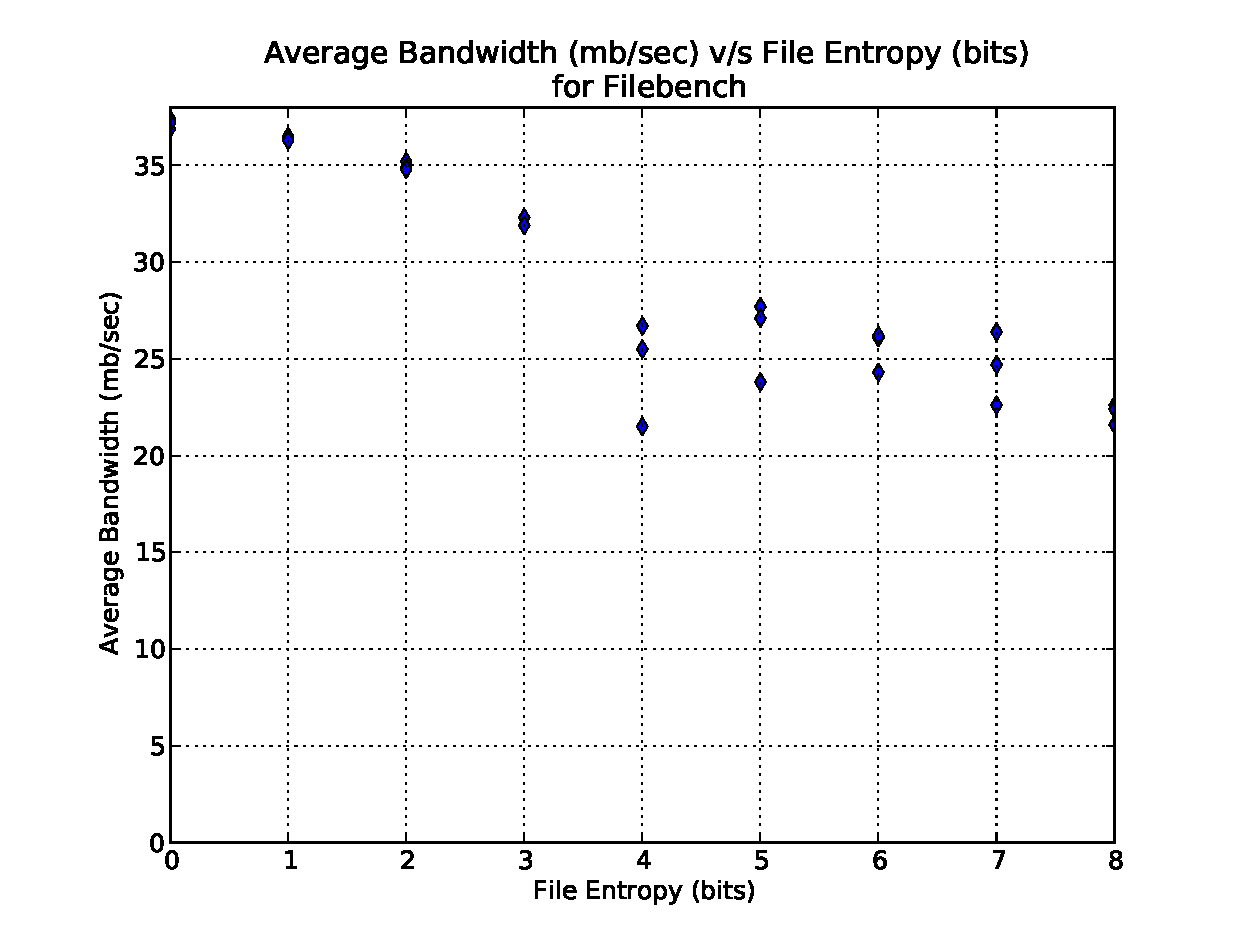
\includegraphics[scale=.55]{../results/write_bw_all.eps}
\caption{The bandwidth of all the write runs}
\end{center}
\end{figure}

\begin{figure}
\label{fig:wbavg}
\begin{center}
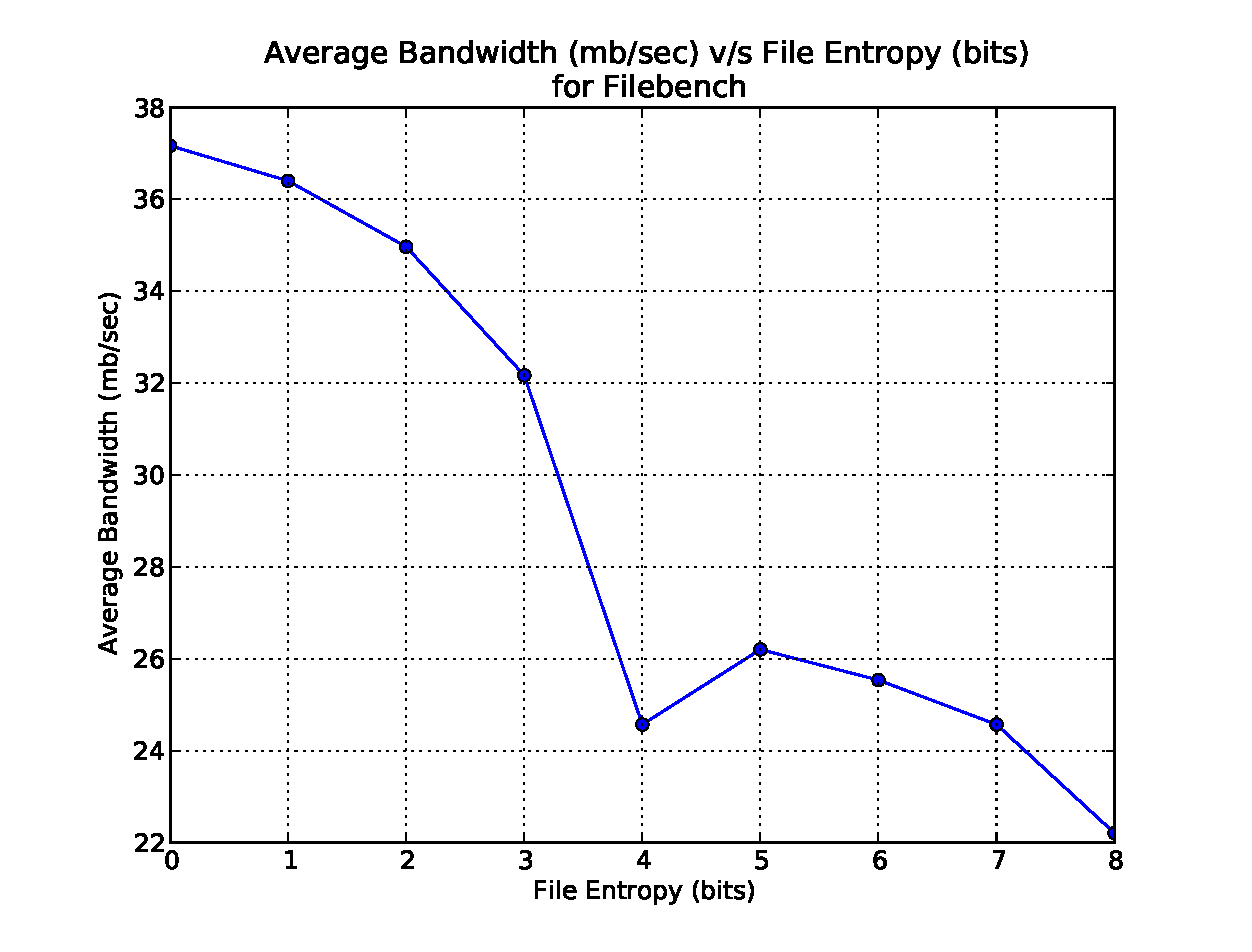
\includegraphics[scale=.55]{../results/write_bw_avg.eps}
\caption{The average bandwidh over all the different write runs}
\end{center}
\end{figure}

\begin{figure}
\label{fig:wl}
\begin{center}
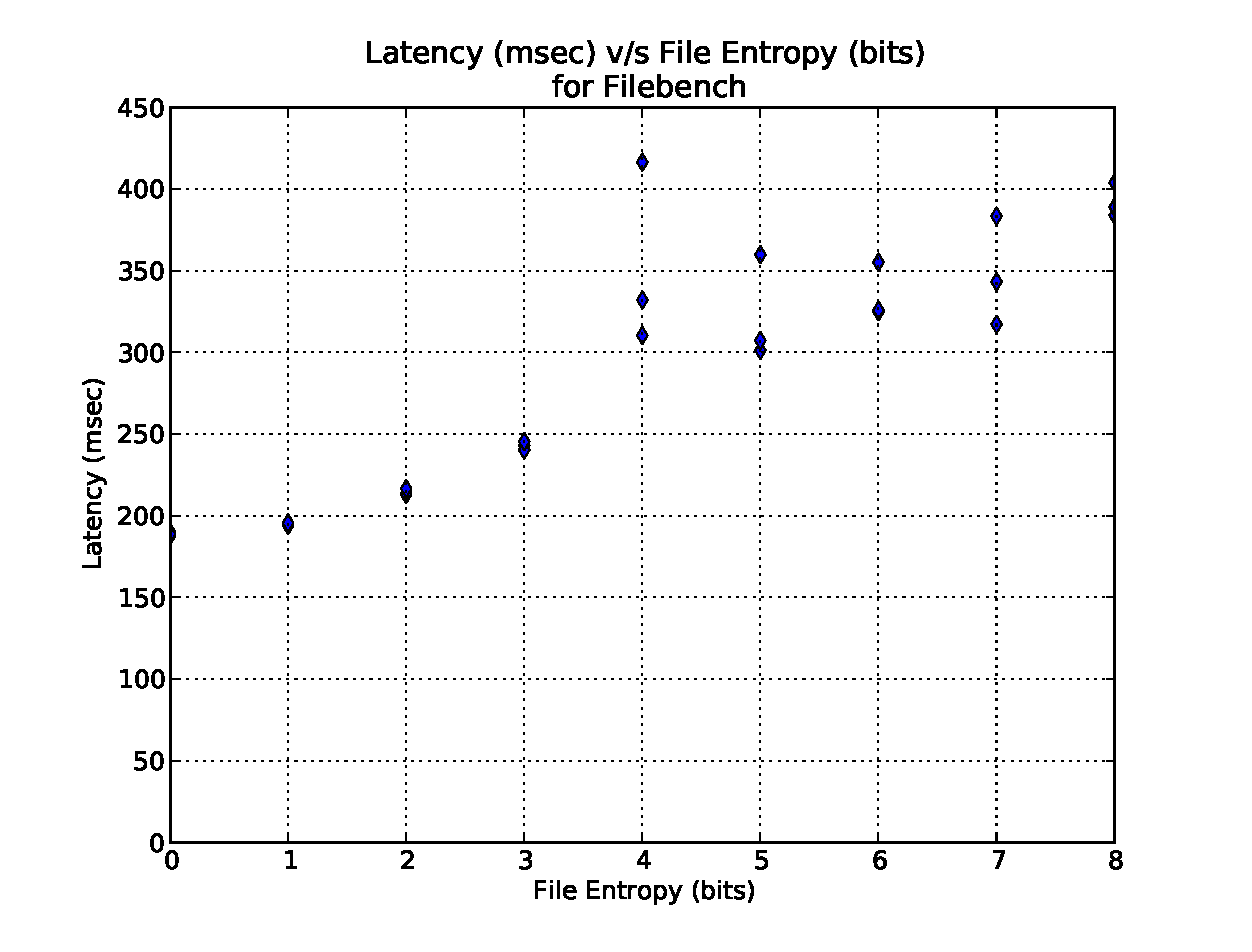
\includegraphics[scale=.55]{../results/write_latency_all.eps}
\caption{The latency of all the different write runs}
\end{center}
\end{figure}


\begin{figure}
\label{fig:wlavg}
\begin{center}
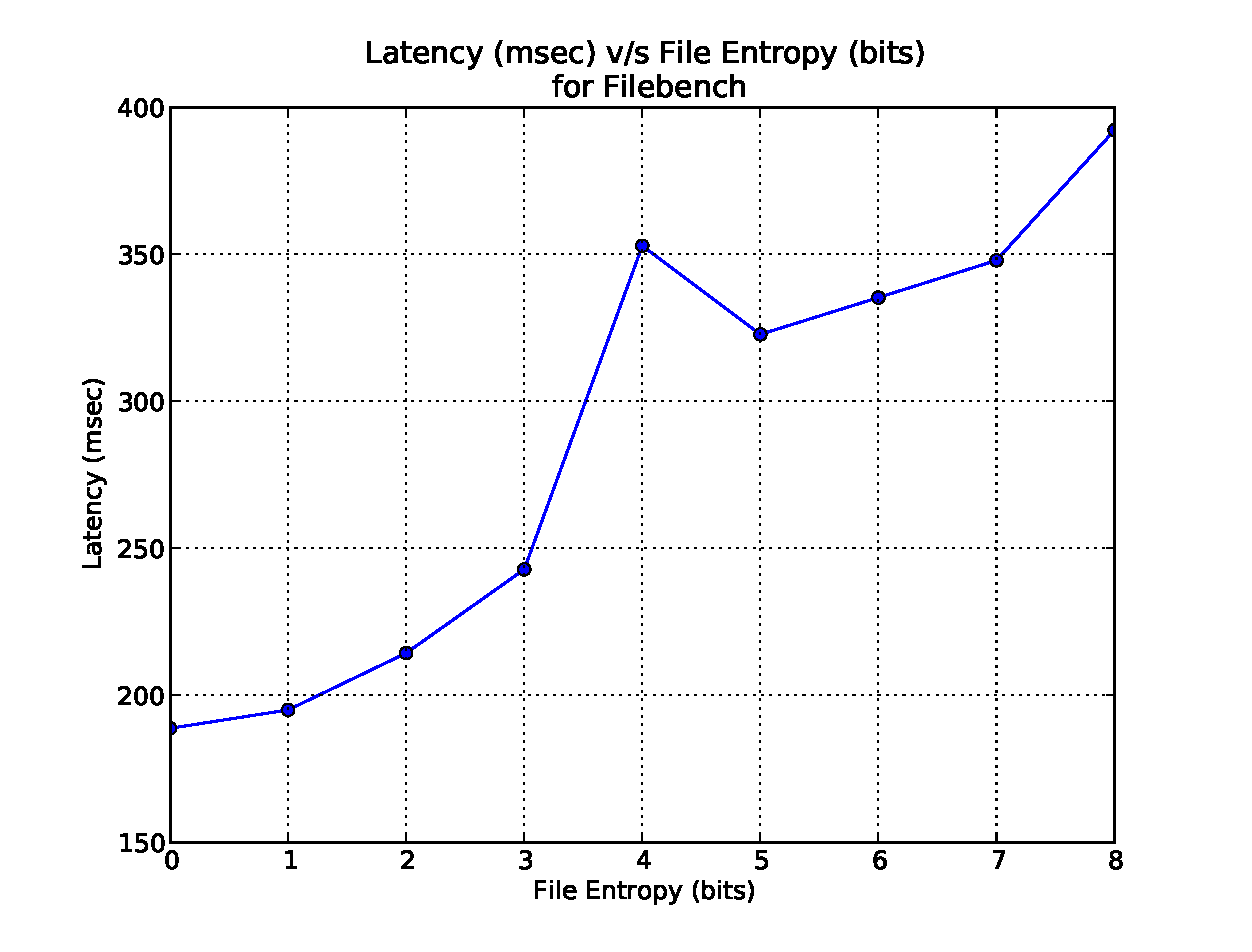
\includegraphics[scale=.55]{../results/write_latency_avg.eps}
\caption{The average latency over all the write runs}
\end{center}
\end{figure}

\begin{figure}
\label{fig:wops}
\begin{center}
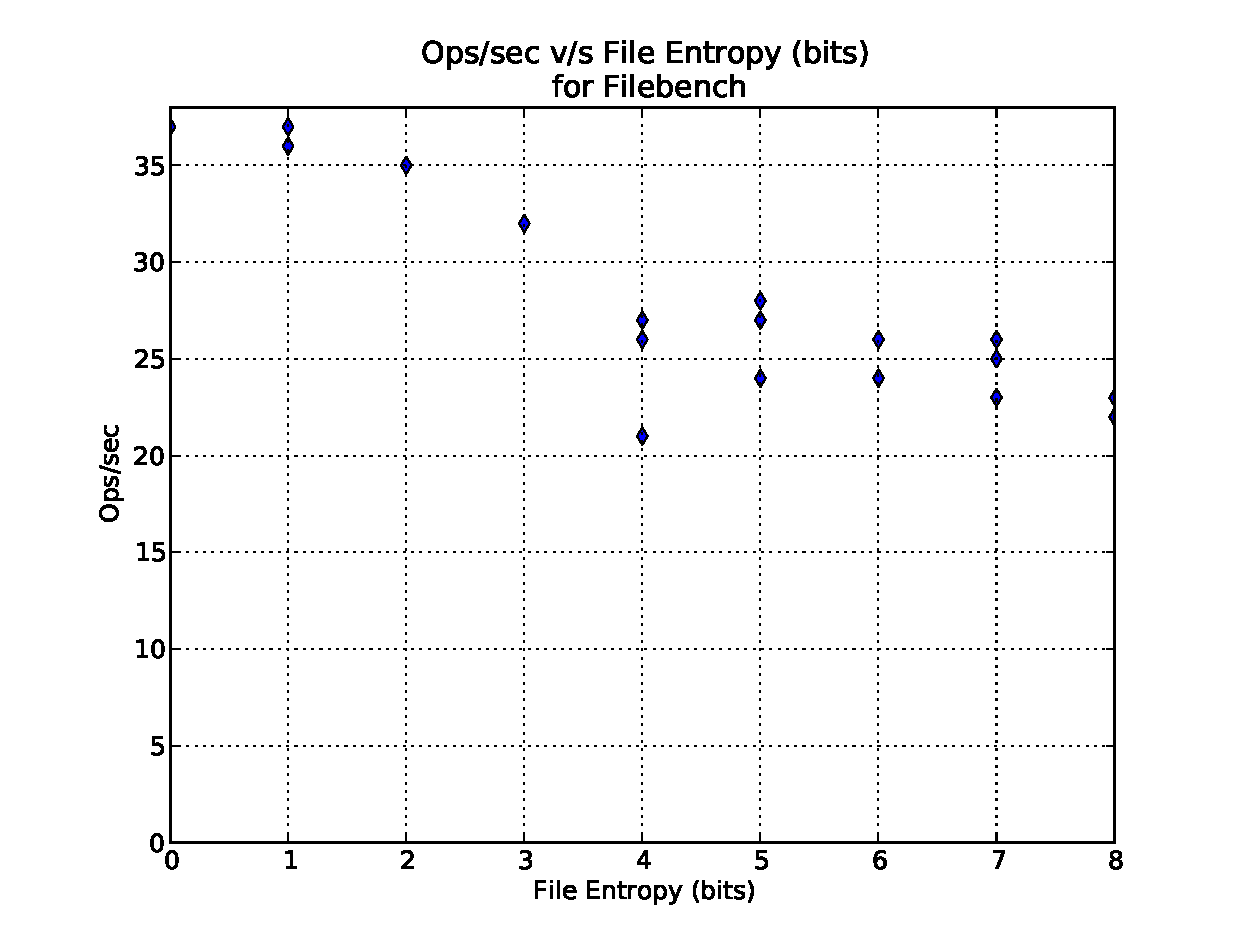
\includegraphics[scale=.55]{../results/write_ops_all.eps}
\caption{The operations execution speed of all the write runs}
\end{center}
\end{figure}


\begin{figure}
\label{fig:wopsavg}
\begin{center}
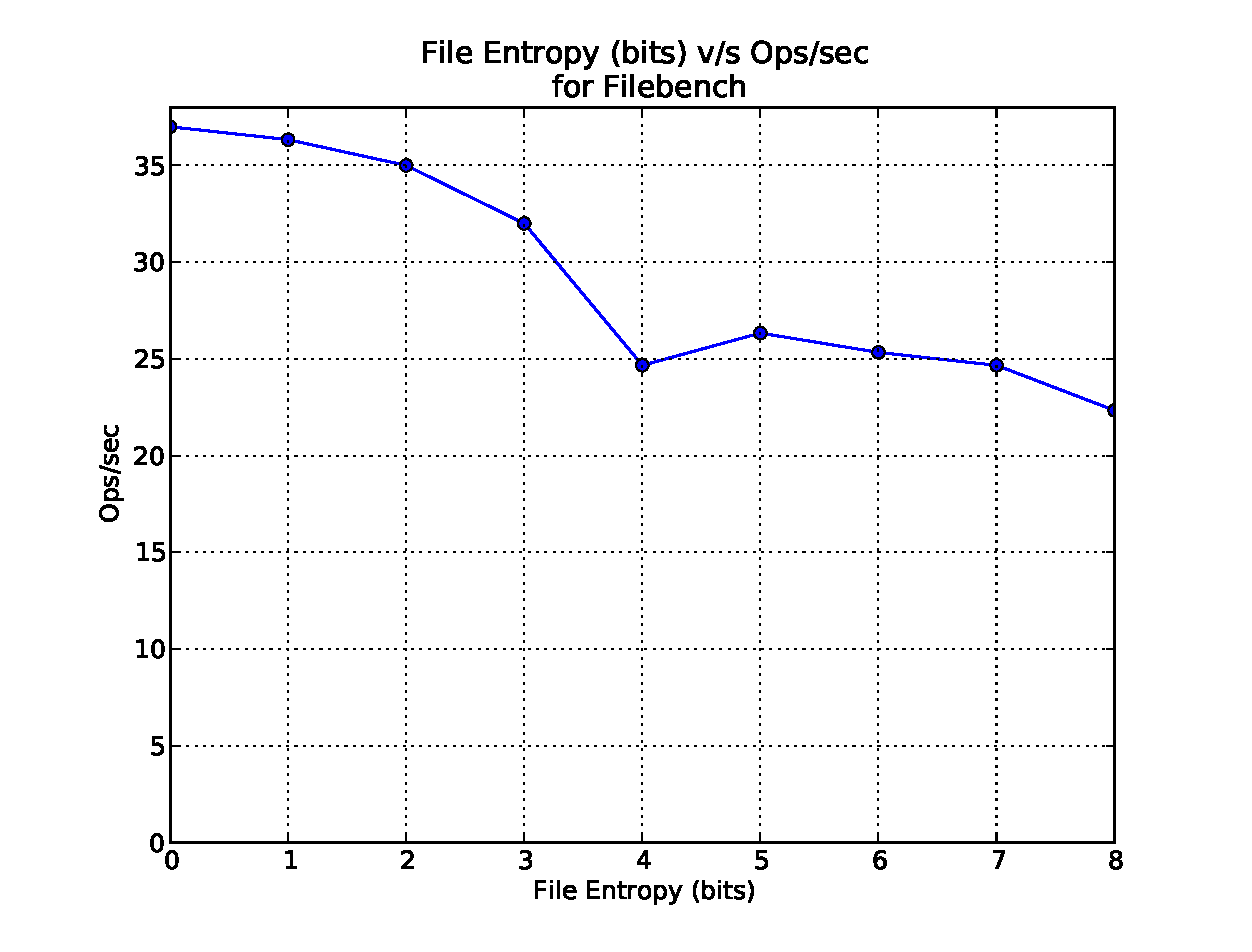
\includegraphics[scale=.55]{../results/write_ops_avg.eps}
\caption{The average operations execution speed over all the write runs}
\end{center}
\end{figure}

\begin{figure}
\label{fig:rb}
\begin{center}
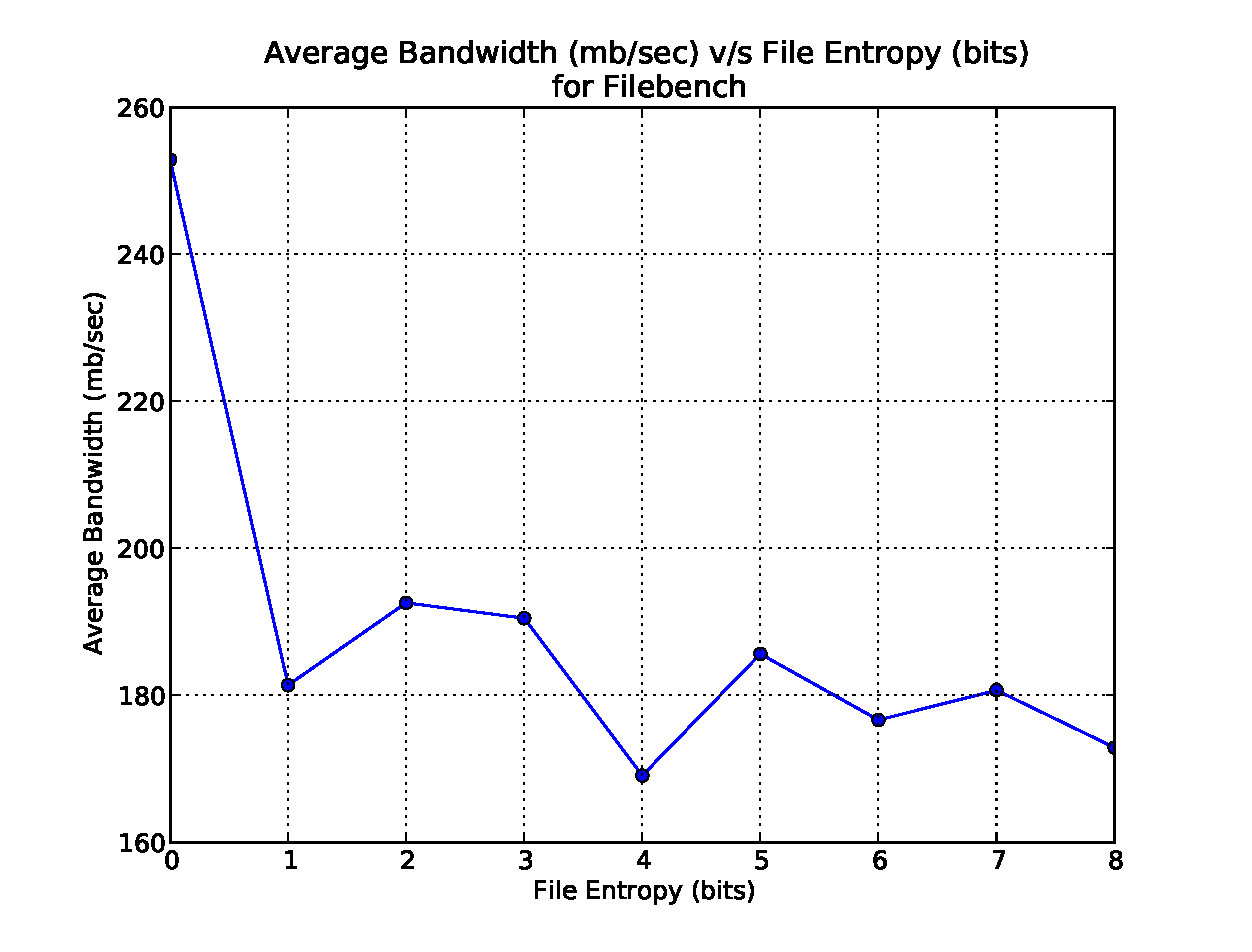
\includegraphics[scale=0.55]{../results/read_bw.eps}
\caption{The bandwidth of all the read runs }
\end{center}
\end{figure}

\begin{figure}
\label{fig:rl}
\begin{center}
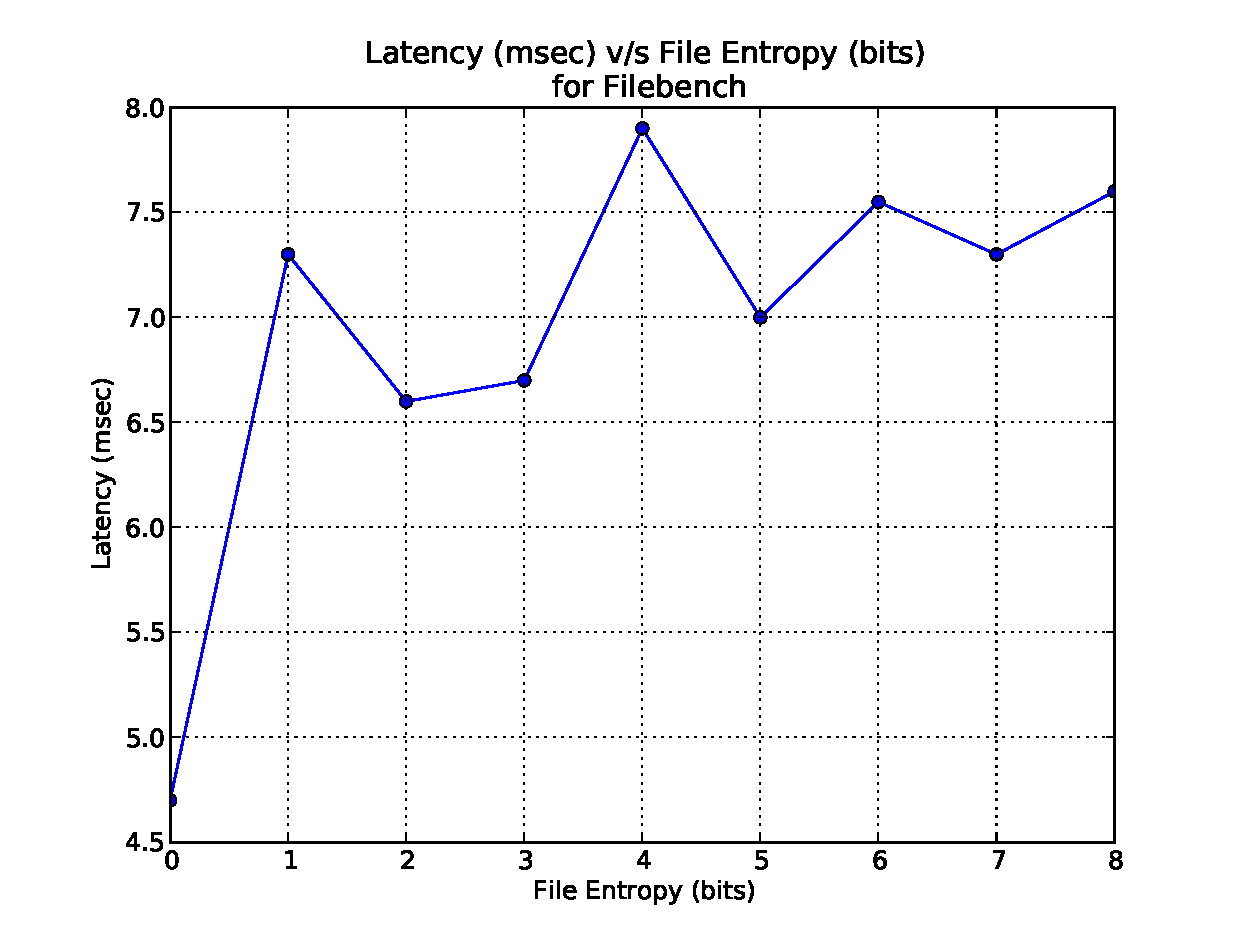
\includegraphics[scale=.55]{../results/read_latency.eps}
\caption{The latency over all the read runs}
\end{center}
\end{figure}


\section{Lookup fill method results}


\chapter{Conclusions}\label{chap:conc}
\chapter{Future Work}\label{chap:fut}


Currently generating the random data takes a lot of time, except for the contiguous method explained in section \ref{sec:ent_imp}.
This makes the processor lags behind the disk, which keeps the disk idle most of the time.
 However, this should not affect the results when we compare the readings obtained from different levels of an entropy used with a deduplication file system.
 However, testing other non-deduplication filesystems with entropy generation enabled will cause unexpected results because of the way the statistics are collected in Filebench.
\paragraph{}
 Filebench calculates the averages bandwidth and operations per second.
 Therefore, if the entropy is enabled while running filebench on ext2 for example, most of the time the disk will be idle which will result in lower readings than the case if entropy is switched off, although ext2 is not aware of the data that is being written the previous scenario 
\paragraph{}
To fix this, Filebench has to be modified to calculate the time the disk is actually used and use only that time to calculate the average bandwidth and operations per second.
\paragraph{}
Another point to mention is the model we are using to model practical loads. We are using entropy as the only characteristics of the file that is actually varied.
 Moreover, it is the same value across all the files. In normal loads like the ones in cloud computing servers where there is a lot of backups and snapshots, the entropy can high per file but the redundancy is also high.
 Using true randomization makes it so hard to generate any chunk of the file twice.
 Maybe it is better to generate a more realistic model by profiling large amount of storage and construct the PDF from that data. We can use such PDF to to calculate the probability that a page will be redundant to one already have been written on the disk.

%-----------------------------------------------------------
\addcontentsline{toc}{chapter}{\numberline{}Bibliography}
\bibliographystyle{plain}
\bibliography{bib}

%-----------------------------------------------------------
\end{document}
